\documentclass[12pt,a4paper]{amsart}
\usepackage[utf8]{inputenc}
\usepackage[T1]{fontenc}
\usepackage{amsmath,amsfonts,amssymb}
\usepackage{tikz}
\usepackage{algorithm}
\usepackage{algorithmic}
\usepackage{float}
\usepackage{listings}
\usepackage{xcolor}
\usepackage{geometry}
\usepackage{fancyhdr}
\usepackage{enumitem}
\usepackage{booktabs}
\usepackage{multirow}
\usepackage{mdframed}
\usepackage[hidelinks,bookmarksnumbered,bookmarksopen]{hyperref}
\usepackage{xeCJK}
\setCJKmainfont{LXGW WenKai}

\geometry{left=2.5cm,right=2.5cm,top=2.5cm,bottom=2.5cm}

% 代码高亮设置
\lstset{
    language=C++,
    basicstyle=\ttfamily\small,
    keywordstyle=\color{blue}\bfseries,
    commentstyle=\color{green!60!black},
    stringstyle=\color{red},
    numbers=left,
    numberstyle=\tiny\color{gray},
    stepnumber=1,
    numbersep=10pt,
    backgroundcolor=\color{gray!10},
    frame=single,
    tabsize=4,
    captionpos=b,
    breaklines=true,
    breakatwhitespace=false,
    showspaces=false,
    showstringspaces=false,
    showtabs=false
}

% 定理环境
\newtheorem{definition}{定义}[section]
\newtheorem{theorem}{定理}[section]
\newtheorem{example}{例题}[section]
\newtheorem{property}{性质}[section]

% TikZ库
\usetikzlibrary{trees,positioning,arrows,automata,calc}

% 定义mdframed样式
\mdfdefinestyle{framestyle}{
    linecolor=blue,
    linewidth=2pt,
    roundcorner=5pt,
    backgroundcolor=blue!10
}

\title{\textbf{数据结构 - 字符串和多维数组复习资料}}
\author{详细版本}
\date{\today}

\begin{document}

\maketitle

% 目录设置
\tableofcontents
\newpage

\subsection{字符串的定义}

\begin{definition}[字符串]
字符串(string)是由 $n(n \geq 0)$ 个字符组成的有限序列,记作:
$$S = "s_1s_2\cdots s_n"$$
其中 $S$ 是串名,双引号是定界符,不属于串的内容,$s_i(1 \leq i \leq n)$ 是一个任意字符,$n$ 为串的长度。$s_i$ 在串中出现的序号称为该字符在串中的位置。
\end{definition}

\subsection{字符串的基本术语}

\begin{definition}[空串]
长度为0的串称为空串,记作"",空串中不包含任何字符。
\end{definition}

\begin{definition}[空格串]
由一个或多个空格组成的串称为空格串,其长度是串中包含的空格数。
\end{definition}

\begin{definition}[子串]
字符串中任意个连续的字符组成的子序列称为该串的子串(substring)。
\end{definition}

\begin{definition}[主串]
包含子串的串称为主串(primary string)。
\end{definition}

\begin{definition}[子串位置]
子串的第一个字符在主串中的序号称为子串在主串中的位置(location)。
\end{definition}

\subsection{字符串的比较}

字符集中的每个字符都有一个唯一的数值表示——称为字符编码,字符间的大小关系就定义为对应字符编码之间的大小关系。

给定两个字符串 $X = "x_1x_2\cdots x_n"$,$Y = "y_1y_2\cdots y_m"$:

\begin{align}
X = Y &\iff n = m \text{ 且 } x_i = y_i \text{ for all } i \\
X < Y &\iff \begin{cases}
n < m \text{ 且 } x_i = y_i (i = 1,2,\ldots,n) \\
\text{或存在 } k \leq \min(m,n) \text{ 使得 } x_i = y_i (i < k), x_k < y_k
\end{cases}
\end{align}

\textbf{例如:}
\begin{itemize}
\item "abcd" = "abcd"
\item "abc" < "abcd"
\item "abac" < "abaec"
\item "aba fg" < "abc"
\end{itemize}

\section{字符串的存储结构}

字符串是数据元素为单个字符的线性表,一般采用顺序存储,即用数组来存储串的字符序列。在C、C++、Java等语言中,字符串都是采用顺序存储。

\subsection{字符串长度的表示方法}

在字符串的顺序存储中,一般有以下三种方法表示串的长度:

\subsubsection{方法一:用变量存储长度}

\begin{center}
\begin{tikzpicture}
\draw (0,0) rectangle (10,0.8);
\foreach \x in {0,1,2,3,4,5,6,7,8,9}
    \draw (\x,0) -- (\x,0.8);
\node at (0.5,0.4) {a};
\node at (1.5,0.4) {b};
\node at (2.5,0.4) {c};
\node at (3.5,0.4) {d};
\node at (4.5,0.4) {e};
\node at (5.5,0.4) {f};
\node at (6.5,0.4) {g};
\node at (7.5,0.4) {h};
\node at (8.5,0.4) {i};
\node at (9.5,0.4) {空闲};
\node at (0.5,-0.3) {0};
\node at (1.5,-0.3) {1};
\node at (2.5,-0.3) {2};
\node at (3.5,-0.3) {3};
\node at (4.5,-0.3) {4};
\node at (5.5,-0.3) {5};
\node at (6.5,-0.3) {6};
\node at (7.5,-0.3) {7};
\node at (8.5,-0.3) {8};
\node at (9.5,-0.3) {$\cdots$};
\node at (12,0.4) {串的长度为9};
\end{tikzpicture}
\end{center}

\subsubsection{方法二:用数组0号单元存放长度}

\begin{center}
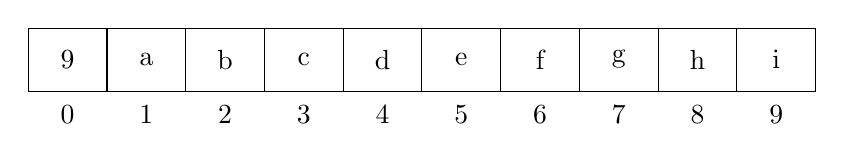
\begin{tikzpicture}
\draw (0,0) rectangle (10,0.8);
\foreach \x in {0,1,2,3,4,5,6,7,8,9}
    \draw (\x,0) -- (\x,0.8);
\node at (0.5,0.4) {9};
\node at (1.5,0.4) {a};
\node at (2.5,0.4) {b};
\node at (3.5,0.4) {c};
\node at (4.5,0.4) {d};
\node at (5.5,0.4) {e};
\node at (6.5,0.4) {f};
\node at (7.5,0.4) {g};
\node at (8.5,0.4) {h};
\node at (9.5,0.4) {i};
\node at (0.5,-0.3) {0};
\node at (1.5,-0.3) {1};
\node at (2.5,-0.3) {2};
\node at (3.5,-0.3) {3};
\node at (4.5,-0.3) {4};
\node at (5.5,-0.3) {5};
\node at (6.5,-0.3) {6};
\node at (7.5,-0.3) {7};
\node at (8.5,-0.3) {8};
\node at (9.5,-0.3) {9};
\end{tikzpicture}
\end{center}

\subsubsection{方法三:用结束符标记}

在串尾存储一个不会在串中出现的特殊字符作为字符串的终结符,例如,在C、C++和Java语言中用'\textbackslash 0'来表示串的结束。

\begin{center}
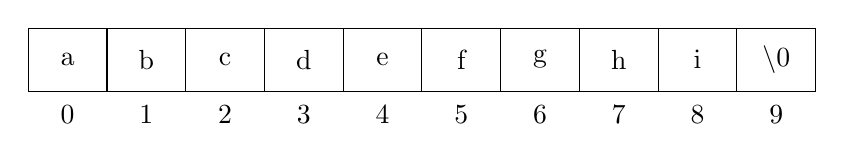
\begin{tikzpicture}
\draw (0,0) rectangle (10,0.8);
\foreach \x in {0,1,2,3,4,5,6,7,8,9}
    \draw (\x,0) -- (\x,0.8);
\node at (0.5,0.4) {a};
\node at (1.5,0.4) {b};
\node at (2.5,0.4) {c};
\node at (3.5,0.4) {d};
\node at (4.5,0.4) {e};
\node at (5.5,0.4) {f};
\node at (6.5,0.4) {g};
\node at (7.5,0.4) {h};
\node at (8.5,0.4) {i};
\node at (9.5,0.4) {\textbackslash 0};
\node at (0.5,-0.3) {0};
\node at (1.5,-0.3) {1};
\node at (2.5,-0.3) {2};
\node at (3.5,-0.3) {3};
\node at (4.5,-0.3) {4};
\node at (5.5,-0.3) {5};
\node at (6.5,-0.3) {6};
\node at (7.5,-0.3) {7};
\node at (8.5,-0.3) {8};
\node at (9.5,-0.3) {9};
\end{tikzpicture}
\end{center}

这种存储方法不能直接得到串的长度,而是通过判断当前字符是否为'\textbackslash 0'来确定串是否结束,从而求得串的长度。

\subsection{字符串的抽象数据类型定义}

字符串的逻辑结构与线性表的逻辑结构相同,但字符串的基本操作和线性表的基本操作有很大差别。线性表的基本操作大多以"单个元素"作为操作对象,而字符串的基本操作通常以"字符串整体"作为操作对象。

\begin{lstlisting}[caption=字符串抽象数据类型]
ADT String {
    数据对象:D = {ai | ai ∈ CharacterSet, i = 1,2,...,n, n ≥ 0}
    数据关系:R1 = {<ai-1, ai> | ai-1, ai ∈ D, i = 2,...,n}
    基本操作:
        StrAssign(T, chars);          // 串赋值
        StrCopy(T, S);               // 串复制
        StrEmpty(S);                 // 判断串空
        StrCompare(S, T);            // 串比较
        StrLength(S);                // 求串长
        StrConcat(T, S1, S2);        // 串连接
        SubString(Sub, S, pos, len); // 求子串
        Index(S, T, pos);            // 子串定位
        Replace(S, T, V);            // 串替换
        StrInsert(S, pos, T);        // 串插入
        StrDelete(S, pos, len);      // 串删除
} ADT String
\end{lstlisting}

\section{模式匹配算法}

模式匹配是字符串处理中最重要的操作之一。给定两个字符串 $S = "s_1s_2\cdots s_n"$ 和 $T = "t_1t_2\cdots t_m"$,在主串 $S$ 中寻找子串 $T$ 的过程称为模式匹配(pattern matching),$T$ 称为模式(pattern)。如果匹配成功,返回 $T$ 在 $S$ 中的位置;如果匹配失败,返回0。

\subsection{BF算法(暴力匹配)}

BF算法(Brute-Force algorithm)的基本思想是蛮力匹配,即从主串 $S$ 的第一个字符开始和模式 $T$ 的第一个字符进行比较。若相等,则继续比较两者的后续字符;否则,从主串 $S$ 的第二个字符开始和模式 $T$ 的第一个字符进行比较。重复上述过程,直至 $S$ 或 $T$ 中所有字符比较完毕。

\begin{algorithm}[H]
\caption{BF算法}
\begin{algorithmic}[1]
\REQUIRE 主串$S$,模式$T$
\ENSURE $T$在$S$中的位置
\STATE $start \leftarrow 0$, $i \leftarrow 0$, $j \leftarrow 0$
\WHILE{$S[i] \neq '\backslash 0'$ AND $T[j] \neq '\backslash 0'$}
    \IF{$S[i] = T[j]$}
        \STATE $i \leftarrow i + 1$, $j \leftarrow j + 1$
    \ELSE
        \STATE $start \leftarrow start + 1$
        \STATE $i \leftarrow start$, $j \leftarrow 0$
    \ENDIF
\ENDWHILE
\IF{$T[j] = '\backslash 0'$}
    \RETURN $start + 1$
\ELSE
    \RETURN $0$
\ENDIF
\end{algorithmic}
\end{algorithm}

\begin{lstlisting}[caption=BF算法C++实现]
int BF(char S[], char T[]) {
    int start = 0;  // 主串从下标0开始第一趟匹配
    int i = 0, j = 0;  // 设置比较的起始下标
    
    while (S[i] != '\0' && T[j] != '\0') {
        if (S[i] == T[j]) {
            i++; j++;  // 继续比较下一对字符
        } else {
            start++;   // 开始下一趟匹配
            i = start; j = 0;  // i和j分别回溯
        }
    }
    
    if (T[j] == '\0')
        return start + 1;  // 返回本趟匹配的起始位置
    else
        return 0;  // 匹配失败
}
\end{lstlisting}

\begin{theorem}[BF算法时间复杂度]
设主串 $S$ 长度为 $n$,模式 $T$ 长度为 $m$,在匹配成功的情况下,考虑两种极端情况:
\begin{enumerate}
\item \textbf{最好情况}:每趟不成功的匹配都发生在模式 $T$ 的第一个字符。平均比较次数为 $\frac{n+m}{2} = O(n+m)$。
\item \textbf{最坏情况}:每趟不成功的匹配都发生在模式 $T$ 的最后一个字符。平均比较次数为 $\frac{m(n-m+2)}{2} = O(n \times m)$。
\item \textbf{平均情况}:$O(n+m)$
\end{enumerate}
其中$n$为主串长度,$m$为模式长度。
\end{theorem}

\begin{example}[BF算法执行过程]
设主串 $S = "abcabcacb"$,模式 $T = "abcac"$,BF算法的匹配过程如下:

\textbf{第1趟匹配:}
\begin{center}
\begin{tabular}{|c|c|c|c|c|c|c|c|c|c|}
\hline
S & a & b & c & a & b & c & a & c & b \\
\hline
T & a & b & c & a & \textcolor{red}{c} &  &  &  &  \\
\hline
\end{tabular}
\end{center}
$i=4, j=4$ 失败,$i$ 回溯到1,$j$ 回溯到0

\textbf{第2趟匹配:}
\begin{center}
\begin{tabular}{|c|c|c|c|c|c|c|c|c|c|}
\hline
S & a & \textcolor{red}{b} & c & a & b & c & a & c & b \\
\hline
T &  & \textcolor{red}{a} &  &  &  &  &  &  &  \\
\hline
\end{tabular}
\end{center}
$i=1, j=0$ 失败,$i$ 回溯到2,$j$ 回溯到0

\textbf{第3趟匹配:}
\begin{center}
\begin{tabular}{|c|c|c|c|c|c|c|c|c|c|}
\hline
S & a & b & \textcolor{red}{c} & a & b & c & a & c & b \\
\hline
T &  &  & \textcolor{red}{a} &  &  &  &  &  &  \\
\hline
\end{tabular}
\end{center}
$i=2, j=0$ 失败,$i$ 回溯到3,$j$ 回溯到0

\textbf{第4趟匹配:}
\begin{center}
\begin{tabular}{|c|c|c|c|c|c|c|c|c|c|}
\hline
S & a & b & c & a & b & c & a & c & b \\
\hline
T &  &  &  & a & b & c & a & c &  \\
\hline
\end{tabular}
\end{center}
$i=8, j=5$,$T$ 中全部字符都比较完毕,匹配成功,返回位置4。
\end{example}

\subsection{KMP算法}

KMP算法是克努思(Knuth)、莫里斯(Morris)和普拉特(Pratt)同时设计的,是对BF算法的重大改进。KMP算法的核心思想是避免主串指针回溯,通过预计算模式的next数组实现高效匹配。

\subsubsection{KMP算法的基本思想}

分析BF算法的执行过程,造成BF算法效率低的原因是回溯,即在某趟匹配失败后,对于主串$S$要回溯到本趟匹配开始字符的下一个字符,模式$T$要回溯到第一个字符,而这些回溯往往是不必要的。

KMP算法希望某趟在$S[i]$和$T[j]$匹配失败后,下标$i$不回溯,下标$j$回溯至某个位置$k$,使得$T[k]$对准$S[i]$继续进行比较。关键问题是如何确定位置$k$。

\begin{definition}[next数组]
模式中的每一个字符$T[j]$都对应一个$k$值,这个$k$值仅依赖于模式本身,与主串无关。用$\text{next}[j]$表示$T[j]$对应的$k$值$(0 \leq j < m)$,其定义如下:
$$\text{next}[j] = \begin{cases}
-1 & j = 0 \\
\max\{k | 1 \leq k < j \text{ 且 } T[0]\cdots T[k-1] = T[j-k]\cdots T[j-1]\} & \text{集合非空} \\
0 & \text{其他情况}
\end{cases}$$
\end{definition}

\textbf{next数组的含义:}
next[j]表示当模式中第j个字符与主串中相应字符"失配"时,在模式中需要重新和主串中该字符进行比较的字符的位置。

\begin{example}[计算next数组]
设模式 $T = "ababc"$,计算其next值:

\begin{center}
\begin{tabular}{|c|c|c|c|c|c|}
\hline
j & 0 & 1 & 2 & 3 & 4 \\
\hline
T[j] & a & b & a & b & c \\
\hline
next[j] & -1 & 0 & 0 & 1 & 2 \\
\hline
\end{tabular}
\end{center}

计算过程:
\begin{itemize}
\item $j=0$: $\text{next}[0] = -1$
\item $j=1$: $\text{next}[1] = 0$
\item $j=2$: $T[0] \neq T[1]$,故 $\text{next}[2] = 0$
\item $j=3$: $T[0] = T[2] = a$,故 $\text{next}[3] = 1$
\item $j=4$: $T[0]T[1] = T[2]T[3] = ab$,故 $\text{next}[4] = 2$
\end{itemize}
\end{example}

\begin{example}[KMP算法执行过程]
设主串 $S = "ababcabcacbab"$,模式 $T = "abcac"$。

首先计算模式T的next数组。`next[j]` 的值是模式串 `T` 的子串 `T[0...j-1]` 的最长公共前后缀的长度。

\begin{center}
\begin{tabular}{|c|c|c|c|c|c|}
\hline
j & 0 & 1 & 2 & 3 & 4 \\
\hline
T[j] & a & b & c & a & c \\
\hline
next[j] & -1 & 0 & 0 & 0 & 1 \\
\hline
\end{tabular}
\end{center}
\textbf{详细计算过程}:
\begin{itemize}
    \item \textbf{j = 0}: 
        \begin{itemize}
            \item `next[0]` 按定义为 -1。这是一个哨兵值,表示模式串的第一个字符就不匹配,此时主串指针需要后移。
        \end{itemize}
    \item \textbf{j = 1}: 
        \begin{itemize}
            \item 子串 `T[0...0]` 为 "a"。
            \item 其所有前缀和后缀都为空。最长公共前后缀长度为0。
            \item 所以 `next[1] = 0`。
        \end{itemize}
    \item \textbf{j = 2}: 
        \begin{itemize}
            \item 子串 `T[0...1]` 为 "ab"。
            \item 前缀: \{"a"\}。后缀: \{"b"\}。
            \item 两者没有交集。最长公共前后缀长度为0。
            \item 所以 `next[2] = 0`。
        \end{itemize}
    \item \textbf{j = 3}: 
        \begin{itemize}
            \item 子串 `T[0...2]` 为 "abc"。
            \item 前缀: \{"a", "ab"\}。后缀: \{"c", "bc"\}。
            \item 两者没有交集。最长公共前后缀长度为0。
            \item 所以 `next[3] = 0`。
        \end{itemize}
    \item \textbf{j = 4}: 
        \begin{itemize}
            \item 子串 `T[0...3]` 为 "abca"。
            \item 前缀: \{"a", "ab", "abc"\}。后缀: \{"a", "ca", "bca"\}。
            \item 最长的公共元素是 "a",长度为1。
            \item 所以 `next[4] = 1`。
        \end{itemize}
\end{itemize}

\textbf{KMP匹配过程} (i为主串指针,j为模式串指针):

\textbf{第1趟匹配:} $i$从0开始, $j$从0开始
\begin{center}
\begin{tabular}{|c|c|c|c|c|c|c|c|c|c|c|c|c|}
\hline
S & a & b & c & a & \textcolor{red}{b} & c & a & c & b & a & b & \\
\hline
T & a & b & c & a & \textcolor{red}{c} &  &  &  &  &  &  &  \\
\hline
索引i & 0 & 1 & 2 & 3 & 4 & 5 & 6 & 7 & 8 & 9 & 10 & 11 \\
\hline
\end{tabular}
\end{center}
在 $i=4, j=4$ 时,$S[4]='b' \neq T[4]='c'$,发生不匹配。\\
根据KMP算法,主串指针$i$不回溯 ($i$保持为4),模式串指针$j$更新为 $j = \text{next}[4] = 1$。

\textbf{第2趟匹配:}
\begin{center}
\begin{tabular}{|c|c|c|c|c|c|c|c|c|c|c|c|c|}
\hline
S & a & b & c & a & \textcolor{red}{b} & c & a & c & b & a & b & \\
\hline
T &   &   &   &   & \textcolor{red}{b} & c & a & c &  &  &  &  \\
\hline
索引i & 0 & 1 & 2 & 3 & 4 & 5 & 6 & 7 & 8 & 9 & 10 & 11 \\
\hline
\end{tabular}
\end{center}
从 $i=4, j=1$ 继续比较。$S[4]='b' = T[1]='b'$,匹配。$i,j$ 都加1。\\
$i=5, j=2$ 时,$S[5]='c' = T[2]='c'$,匹配。$i,j$ 都加1。\\
$i=6, j=3$ 时,$S[6]='a' = T[3]='a'$,匹配。$i,j$ 都加1。\\
$i=7, j=4$ 时,$S[7]='c' = T[4]='c'$,匹配。$i,j$ 都加1。\\
$i=8, j=5$ 时,$T[j]$ 到达末尾($\backslash 0$),说明匹配成功。\\
返回匹配开始的位置 $i-j = 8-5 = 3$ (若从1开始计数,则是位置4)。
\end{example}

\begin{algorithm}
\caption{KMP算法}
\begin{algorithmic}[1]
\REQUIRE 主串$S$,模式$T$,next数组
\ENSURE $T$在$S$中的位置
\STATE $i \leftarrow 0$, $j \leftarrow 0$
\WHILE{$S[i] \neq '\backslash 0'$ AND $T[j] \neq '\backslash 0'$}
    \IF{$S[i] = T[j]$}
        \STATE $i \leftarrow i + 1$, $j \leftarrow j + 1$
    \ELSE
        \STATE $j \leftarrow \text{next}[j]$
        \IF{$j = -1$}
            \STATE $i \leftarrow i + 1$, $j \leftarrow 0$
        \ENDIF
    \ENDIF
\ENDWHILE
\IF{$T[j] = '\backslash 0'$}
    \RETURN $i - j + 1$
\ELSE
    \RETURN $0$
\ENDIF
\end{algorithmic}
\end{algorithm}

\begin{theorem}[KMP算法时间复杂度]
KMP算法的时间复杂度为 $O(n+m)$,其中$n$为主串长度,$m$为模式长度。
\end{theorem}

\section{多维数组}

\subsection{数组的基本概念}

\begin{definition}[数组]
数组是由类型相同的数据元素构成的有序集合,每个元素受$n(n \geq 1)$个线性关系约束,每个元素在$n$个线性关系中的序号称为下标。
\end{definition}

数组的特点:
\begin{itemize}
\item 数据元素类型相同
\item 结构固定,一般不做插入删除操作
\item 支持随机访问
\item 是线性表的推广
\end{itemize}

\subsection{数组的存储结构与寻址}

\subsubsection{二维数组的存储}

二维数组可按两种方式存储:
\begin{itemize}
\item \textbf{按行优先}:先行后列存储
\item \textbf{按列优先}:先列后行存储
\end{itemize}

\begin{theorem}[二维数组按行优先寻址公式]
设二维数组$A[l_1..h_1][l_2..h_2]$,按行优先存储,则元素$a_{ij}$的地址为:
$$\text{LOC}(a_{ij}) = \text{LOC}(a_{l_1l_2}) + [(i-l_1) \times (h_2-l_2+1) + (j-l_2)] \times c$$
其中$c$为每个元素占用的存储单元数。
\end{theorem}

\subsubsection{多维数组的寻址}

对于$n$维数组$A[d_1][d_2]\cdots[d_n]$,按行优先存储,元素$A[i_1][i_2]\cdots[i_n]$的地址为:
$$\text{LOC}(A[i_1][i_2]\cdots[i_n]) = \text{LOC}(A[0][0]\cdots[0]) + \left(\sum_{k=1}^{n} i_k \prod_{j=k+1}^{n} d_j\right) \times c$$

\section{矩阵的压缩存储}

\subsection{特殊矩阵的压缩存储}

\subsubsection{对称矩阵}

对称矩阵满足 $a_{ij} = a_{ji}$,只需存储下三角部分。

\begin{theorem}[对称矩阵寻址公式]
$n$阶对称矩阵按行优先存储下三角部分,元素$a_{ij}$在一维数组中的下标为:
$$k = \begin{cases}
\frac{i(i-1)}{2} + j - 1 & \text{if } i \geq j \\
\frac{j(j-1)}{2} + i - 1 & \text{if } i < j
\end{cases}$$
\end{theorem}

\subsubsection{三角矩阵}

\begin{itemize}
\item \textbf{下三角矩阵}:主对角线以上元素为常数$c$
\item \textbf{上三角矩阵}:主对角线以下元素为常数$c$
\end{itemize}

存储方案:存储非常数元素 + 一个常数。

\subsubsection{对角矩阵(带状矩阵)}

对角矩阵的非零元素集中在主对角线及其附近的几条对角线上。

\begin{example}[三对角矩阵]
三对角矩阵的寻址公式:
$$k = 2i + j - 3 \quad (|i-j| \leq 1)$$
\end{example}

\subsection{稀疏矩阵的存储}

\begin{definition}[稀疏矩阵]
设$m \times n$矩阵中有$t$个非零元素,若$t \ll m \times n$,则称该矩阵为稀疏矩阵。
\end{definition}

稀疏矩阵的存储策略:只存储非零元素,节省存储空间。

\subsubsection{三元组表示法}

三元组$(i, j, v)$表示矩阵第$i$行第$j$列的元素值为$v$。

\begin{lstlisting}[caption=三元组结构定义]
typedef struct {
    int i, j;        // 行号和列号
    ElemType e;      // 元素值
} Triple;

typedef struct {
    Triple data[MAXSIZE];  // 三元组表
    int m, n, t;          // 矩阵的行数、列数和非零元素个数
} TSMatrix;
\end{lstlisting}

\subsubsection{稀疏矩阵的转置}

\textbf{方法一:简单转置算法}

\begin{algorithm}[H]
\caption{简单转置算法}
\begin{algorithmic}[1]
\REQUIRE 稀疏矩阵$A$
\ENSURE 转置矩阵$B$
\STATE $B.m \leftarrow A.n$, $B.n \leftarrow A.m$, $B.t \leftarrow A.t$
\STATE $q \leftarrow 1$
\FOR{$col = 1$ to $A.n$}
    \FOR{$p = 1$ to $A.t$}
        \IF{$A.data[p].j = col$}
            \STATE $B.data[q].i \leftarrow A.data[p].j$
            \STATE $B.data[q].j \leftarrow A.data[p].i$
            \STATE $B.data[q].e \leftarrow A.data[p].e$
            \STATE $q \leftarrow q + 1$
        \ENDIF
    \ENDFOR
\ENDFOR
\end{algorithmic}
\end{algorithm}

\begin{theorem}[简单转置算法时间复杂度]
时间复杂度为$O(n \times t)$,其中$n$为矩阵列数,$t$为非零元素个数。当$t$与$m \times n$同数量级时,算法的时间复杂度为$O(m \times n^2)$。
\end{theorem}

\textbf{方法二:快速转置算法}

利用辅助数组记录每列的非零元素个数和每列第一个非零元素在转置矩阵中的位置。

\begin{algorithm}[H]
\caption{快速转置算法}
\begin{algorithmic}[1]
\REQUIRE 稀疏矩阵$A$
\ENSURE 转置矩阵$B$
\STATE $B.m \leftarrow A.n$, $B.n \leftarrow A.m$, $B.t \leftarrow A.t$
\STATE 初始化$num[1..A.n]$和$cpot[1..A.n]$
\FOR{$col = 1$ to $A.n$}
    \STATE $num[col] \leftarrow 0$
\ENDFOR
\FOR{$t = 1$ to $A.t$}
    \STATE $num[A.data[t].j] \leftarrow num[A.data[t].j] + 1$
\ENDFOR
\STATE $cpot[1] \leftarrow 1$
\FOR{$col = 2$ to $A.n$}
    \STATE $cpot[col] \leftarrow cpot[col-1] + num[col-1]$
\ENDFOR
\FOR{$p = 1$ to $A.t$}
    \STATE $col \leftarrow A.data[p].j$
    \STATE $pos \leftarrow cpot[col]$
    \STATE $B.data[pos] \leftarrow$ 转置$A.data[p]$
    \STATE $cpot[col] \leftarrow cpot[col] + 1$
\ENDFOR
\end{algorithmic}
\end{algorithm}

\begin{theorem}[快速转置算法时间复杂度]
时间复杂度为$O(n + t)$,其中$n$为矩阵列数,$t$为非零元素个数。
\end{theorem}

\subsubsection{十字链表表示法}

对于频繁进行插入、删除操作的稀疏矩阵,三元组表示法效率较低,可采用十字链表表示法。

\begin{lstlisting}[caption=十字链表结构定义]
typedef struct OLNode {
    int i, j;                    // 行号和列号
    ElemType e;                  // 元素值
    struct OLNode *right, *down; // 同行右邻接和同列下邻接
} OLNode, *OLink;

typedef struct {
    OLink *rhead, *chead;  // 行和列链表头指针向量
    int m, n, t;          // 矩阵的行数、列数和非零元素个数
} CrossList;
\end{lstlisting}

十字链表的优点:
\begin{itemize}
\item 能够方便地进行按行或按列遍历
\item 插入和删除操作效率高
\item 适合于矩阵运算
\end{itemize}

\subsubsection{稀疏矩阵转置算法详细示例}

设有如下$6 \times 7$稀疏矩阵$A$,包含7个非零元素:

$$
A = \begin{pmatrix}
0 & 0 & 12 & 0 & 9 & 0 & 0 \\
0 & 0 & 0 & 0 & 0 & 0 & 0 \\
0 & -1 & 0 & 0 & 0 & 0 & 0 \\
5 & 0 & 0 & -3 & 0 & 0 & 0 \\
0 & 0 & 0 & 0 & 0 & 2 & 0 \\
0 & 0 & 0 & 0 & 8 & 0 & 0
\end{pmatrix}
$$

三元组表示为:$A.m = 6$,$A.n = 7$,$A.t = 7$

\begin{center}
\begin{tabular}{|c|c|c|c|}
\hline
p(下标) & i(行) & j(列) & e(值) \\
\hline
1 & 1 & 3 & 12 \\
2 & 1 & 5 & 9 \\
3 & 3 & 2 & -1 \\
4 & 4 & 1 & 5 \\
5 & 4 & 4 & -3 \\
6 & 5 & 6 & 2 \\
7 & 6 & 5 & 8 \\
\hline
\end{tabular}
\end{center}

\textbf{例:简单转置算法执行过程}

初始化:$B.m = 7$,$B.n = 6$,$B.t = 7$,$q = 1$

\begin{enumerate}
\item \textbf{col = 1}:扫描$A.data$,找到$A.data[4]$的$j=1$
    \begin{itemize}
    \item 转置$(4, 1, 5) \rightarrow (1, 4, 5)$
    \item 存入$B.data[1]$,$q = 2$
    \end{itemize}

\item \textbf{col = 2}:扫描$A.data$,找到$A.data[3]$的$j=2$
    \begin{itemize}
    \item 转置$(3, 2, -1) \rightarrow (2, 3, -1)$
    \item 存入$B.data[2]$,$q = 3$
    \end{itemize}

\item \textbf{col = 3}:扫描$A.data$,找到$A.data[1]$的$j=3$
    \begin{itemize}
    \item 转置$(1, 3, 12) \rightarrow (3, 1, 12)$
    \item 存入$B.data[3]$,$q = 4$
    \end{itemize}

\item \textbf{col = 4}:扫描$A.data$,找到$A.data[5]$的$j=4$
    \begin{itemize}
    \item 转置$(4, 4, -3) \rightarrow (4, 4, -3)$
    \item 存入$B.data[4]$,$q = 5$
    \end{itemize}

\item \textbf{col = 5}:扫描$A.data$,找到两个元素$j=5$
    \begin{itemize}
    \item 转置$(1, 5, 9) \rightarrow (5, 1, 9)$,存入$B.data[5]$,$q = 6$
    \item 转置$(6, 5, 8) \rightarrow (5, 6, 8)$,存入$B.data[6]$,$q = 7$
    \end{itemize}

\item \textbf{col = 6}:扫描$A.data$,找到$A.data[6]$的$j=6$
    \begin{itemize}
    \item 转置$(5, 6, 2) \rightarrow (6, 5, 2)$
    \item 存入$B.data[7]$,$q = 8$
    \end{itemize}

\item \textbf{col = 7}:扫描$A.data$,无元素
\end{enumerate}

\textbf{最终结果$B.data$:}

\begin{center}
\begin{tabular}{|c|c|c|c|}
\hline
q(下标) & i(行) & j(列) & e(值) \\
\hline
1 & 1 & 4 & 5 \\
2 & 2 & 3 & -1 \\
3 & 3 & 1 & 12 \\
4 & 4 & 4 & -3 \\
5 & 5 & 1 & 9 \\
6 & 5 & 6 & 8 \\
7 & 6 & 5 & 2 \\
\hline
\end{tabular}
\end{center}

\textbf{例:快速转置算法执行过程}

\textbf{步骤1:计算num数组}

$num[col]$存储$A$的第$col$列的非零元素个数。扫描$A.data$一次:

\begin{center}
\begin{tabular}{|c|c|c|c|c|c|c|c|}
\hline
col & 1 & 2 & 3 & 4 & 5 & 6 & 7 \\
\hline
num & 1 & 1 & 1 & 1 & 2 & 1 & 0 \\
\hline
\end{tabular}
\end{center}

\textbf{步骤2:计算cpot数组}

$cpot[col]$存储$A$的第$col$列元素在$B.data$中的起始位置:

\begin{align}
cpot[1] &= 1 \\
cpot[2] &= cpot[1] + num[1] = 1 + 1 = 2 \\
cpot[3] &= cpot[2] + num[2] = 2 + 1 = 3 \\
cpot[4] &= cpot[3] + num[3] = 3 + 1 = 4 \\
cpot[5] &= cpot[4] + num[4] = 4 + 1 = 5 \\
cpot[6] &= cpot[5] + num[5] = 5 + 2 = 7 \\
cpot[7] &= cpot[6] + num[6] = 7 + 1 = 8
\end{align}

\begin{center}
\begin{tabular}{|c|c|c|c|c|c|c|c|}
\hline
col & 1 & 2 & 3 & 4 & 5 & 6 & 7 \\
\hline
cpot & 1 & 2 & 3 & 4 & 5 & 7 & 8 \\
\hline
\end{tabular}
\end{center}

\textbf{步骤3:放置元素到$B.data$}

最后一次扫描$A.data$,对每个元素$A.data[p]$:

\begin{enumerate}
\item \textbf{p = 1}:$A.data[1] = (1, 3, 12)$,$col=3$,$pos = cpot[3] = 3$
    \begin{itemize}
    \item 放置$(3, 1, 12)$到$B.data[3]$
    \item $cpot[3] \leftarrow 4$
    \end{itemize}

\item \textbf{p = 2}:$A.data[2] = (1, 5, 9)$,$col=5$,$pos = cpot[5] = 5$
    \begin{itemize}
    \item 放置$(5, 1, 9)$到$B.data[5]$
    \item $cpot[5] \leftarrow 6$
    \end{itemize}

\item \textbf{p = 3}:$A.data[3] = (3, 2, -1)$,$col=2$,$pos = cpot[2] = 2$
    \begin{itemize}
    \item 放置$(2, 3, -1)$到$B.data[2]$
    \item $cpot[2] \leftarrow 3$
    \end{itemize}

\item \textbf{p = 4}:$A.data[4] = (4, 1, 5)$,$col=1$,$pos = cpot[1] = 1$
    \begin{itemize}
    \item 放置$(1, 4, 5)$到$B.data[1]$
    \item $cpot[1] \leftarrow 2$
    \end{itemize}

\item \textbf{p = 5}:$A.data[5] = (4, 4, -3)$,$col=4$,$pos = cpot[4] = 4$
    \begin{itemize}
    \item 放置$(4, 4, -3)$到$B.data[4]$
    \item $cpot[4] \leftarrow 5$
    \end{itemize}

\item \textbf{p = 6}:$A.data[6] = (5, 6, 2)$,$col=6$,$pos = cpot[6] = 7$
    \begin{itemize}
    \item 放置$(6, 5, 2)$到$B.data[7]$
    \item $cpot[6] \leftarrow 8$
    \end{itemize}

\item \textbf{p = 7}:$A.data[7] = (6, 5, 8)$,$col=5$,$pos = cpot[5] = 6$
    \begin{itemize}
    \item 放置$(5, 6, 8)$到$B.data[6]$
    \item $cpot[5] \leftarrow 7$
    \end{itemize}
\end{enumerate}

\textbf{最终$B.data$结果:}

\begin{center}
\begin{tabular}{|c|c|c|c|}
\hline
q(下标) & i(行) & j(列) & e(值) \\
\hline
1 & 1 & 4 & 5 \\
2 & 2 & 3 & -1 \\
3 & 3 & 1 & 12 \\
4 & 4 & 4 & -3 \\
5 & 5 & 1 & 9 \\
6 & 5 & 6 & 8 \\
7 & 6 & 5 & 2 \\
\hline
\end{tabular}
\end{center}

两种算法得到相同的结果,但快速转置算法通过预计算避免了重复扫描,大大提高了效率。

\begin{lstlisting}[caption=快速转置算法C++实现]
void FastTranspose(TSMatrix A, TSMatrix &B) {
    B.m = A.n; B.n = A.m; B.t = A.t;
    
    int num[A.n + 1];  // 各列非零元个数
    int cpot[A.n + 1]; // 各列第一个非零元在B中的位置
    
    // 初始化num数组
    for (int col = 1; col <= A.n; col++)
        num[col] = 0;
    
    // 统计各列非零元个数
    for (int t = 1; t <= A.t; t++)
        num[A.data[t].j]++;
    
    // 计算各列第一个非零元在B中的位置
    cpot[1] = 1;
    for (int col = 2; col <= A.n; col++)
        cpot[col] = cpot[col-1] + num[col-1];
    
    // 转置
    for (int p = 1; p <= A.t; p++) {
        int col = A.data[p].j;
        int pos = cpot[col];
        B.data[pos].i = A.data[p].j;
        B.data[pos].j = A.data[p].i;
        B.data[pos].e = A.data[p].e;
        cpot[col]++;
    }
}
\end{lstlisting}

\section{广义表}

\subsection{广义表的定义}

\begin{definition}[广义表]
广义表(Generalized List)是$n(n \geq 0)$个元素的有限序列,记作:
$$LS = (a_1, a_2, \ldots, a_n)$$
其中$LS$是广义表的名称,$a_i$可以是原子或子表。
\end{definition}

\subsection{广义表的特性}

\begin{enumerate}
\item \textbf{有序性}:元素有先后次序
\item \textbf{长度}:最外层包含元素的个数
\item \textbf{深度}:括号的重数
\item \textbf{递归性}:广义表可以为自身的子表
\item \textbf{共享性}:可以被其他广义表所共享
\end{enumerate}

\begin{example}[广义表示例]
\begin{align}
A &= () && \text{空表,长度为0,深度为1} \\
B &= (e) && \text{长度为1,深度为1} \\
C &= (a, (b, c)) && \text{长度为2,深度为2} \\
D &= (a, b, (c, d), e) && \text{长度为4,深度为2} \\
E &= ((a, b), (c, d)) && \text{长度为2,深度为2} \\
F &= (a, F) && \text{递归定义,长度为2,深度无穷}
\end{align}
\end{example}

\subsection{广义表的存储结构}

\subsubsection{头尾链表存储}

\indent

\begin{lstlisting}[caption=头尾链表结构定义]
typedef enum {ATOM, LIST} ElemTag;

typedef struct GLNode {
    ElemTag tag;           // 标志域:ATOM或LIST
    union {
        AtomType atom;     // 原子结点的值域
        struct {
            struct GLNode *hp, *tp;  // 表结点的指针域,hp指向表头,tp指向表尾
        } ptr;
    };
} *GList;
\end{lstlisting}

\subsubsection{子表结点存储}

\indent

\begin{lstlisting}[caption=子表结点结构定义]
typedef struct GLNode {
    ElemTag tag;
    union {
        AtomType atom;
        struct GLNode *hp;  // 指向子表
    };
    struct GLNode *tp;      // 指向同层下一个结点
} *GList;
\end{lstlisting}

\subsection{广义表的基本操作}

\textbf{求广义表的长度:}
\begin{lstlisting}[caption=求广义表长度]
int GListLength(GList L) {
    if (!L) return 0;
    int len = 0;
    while (L) {
        len++;
        L = L->tp;
    }
    return len;
}
\end{lstlisting}

\textbf{求广义表的深度:}
\begin{lstlisting}[caption=求广义表深度]
int GListDepth(GList L) {
    if (!L) return 1;     // 空表深度为1
    if (L->tag == ATOM) return 0;  // 原子深度为0
    
    int maxdep = 0;
    while (L) {
        if (L->tag == LIST) {
            int dep = GListDepth(L->ptr.hp);
            if (dep > maxdep) maxdep = dep;
        }
        L = L->ptr.tp;
    }
    return maxdep + 1;
}
\end{lstlisting}

\subsection{稀疏矩阵的压缩存储}

稀疏矩阵是零元素很多的矩阵,稀疏因子$\delta = \frac{t}{m \times n} < 0.05$。

\subsubsection{三元组顺序表}

将非零元素表示为三元组$(i, j, a_{ij})$,按行优先顺序存储。

\begin{verbatim}
struct Element {
    int row, col;
    DataType value;
};

struct SparseMatrix {
    Element data[MaxSize];
    int rows, cols, nums;  // 行数、列数、非零元个数
};
\end{verbatim}

\subsubsection{十字链表}

每个非零元素节点包含5个域:row, col, value, right, down。
\begin{itemize}
\item right指向同行下一个非零元素
\item down指向同列下一个非零元素
\end{itemize}

\subsection{稀疏矩阵转置算法}

\subsubsection{转置算法1(直接转置)}

\begin{algorithm}
\caption{稀疏矩阵转置算法1}
\begin{algorithmic}[1]
\REQUIRE 稀疏矩阵$A$
\ENSURE 转置矩阵$B$
\STATE 设置$B$的行数、列数、非零元个数
\FOR{$col = 1$ to $A.cols$}
    \FOR{$i = 0$ to $A.nums-1$}
        \IF{$A.data[i].col = col$}
            \STATE 将$A.data[i]$行列交换后存入$B$
        \ENDIF
    \ENDFOR
\ENDFOR
\end{algorithmic}
\end{algorithm}

时间复杂度:$O(cols \times nums)$

\subsubsection{转置算法2(快速转置)}

引入辅助数组:
\begin{itemize}
\item $num[1..A.n]$:第$col$列非零元个数
\item $cpot[1..A.n]$:第$col$列第一个非零元在$B$中的位置
\end{itemize}

递推关系:
$$\begin{cases}
cpot[1] = 0 \\
cpot[col] = cpot[col-1] + num[col-1] \quad (2 \leq col \leq nu)
\end{cases}$$

\begin{algorithm}
\caption{稀疏矩阵转置算法2}
\begin{algorithmic}[1]
\REQUIRE 稀疏矩阵$A$
\ENSURE 转置矩阵$B$
\STATE 统计每列非零元个数到$num[]$
\STATE 计算每列第一个元素在$B$中位置到$cpot[]$
\FOR{$i = 0$ to $A.nums-1$}
    \STATE $col \leftarrow A.data[i].col$
    \STATE $pos \leftarrow cpot[col]$
    \STATE $B.data[pos] \leftarrow$ 转置$A.data[i]$
    \STATE $cpot[col] \leftarrow cpot[col] + 1$
\ENDFOR
\end{algorithmic}
\end{algorithm}

时间复杂度:$O(cols + nums)$

\section{重难点分析}

\subsection{重点内容}
\begin{enumerate}
\item \textbf{模式匹配算法}(★★★★★)
    \begin{itemize}
    \item BF算法的执行过程和复杂度分析
    \item KMP算法的next数组计算
    \item KMP算法的匹配过程
    \end{itemize}
    
\item \textbf{数组寻址公式}(★★★★☆)
    \begin{itemize}
    \item 二维数组按行/列优先的寻址公式
    \item 多维数组的寻址公式推导
    \end{itemize}
    
\item \textbf{特殊矩阵压缩存储}(★★★★☆)
    \begin{itemize}
    \item 对称矩阵的存储和寻址
    \item 三角矩阵的存储方案
    \item 对角矩阵的压缩存储
    \end{itemize}
\end{enumerate}

\subsection{难点内容}
\begin{enumerate}
\item \textbf{KMP算法的next数组计算}(★★★★★)
    \begin{itemize}
    \item 理解next数组的含义
    \item 掌握手工计算next值的方法
    \item 理解KMP算法避免回溯的原理
    \end{itemize}
    
\item \textbf{稀疏矩阵的压缩存储}(★★★★☆)
    \begin{itemize}
    \item 三元组表的组织方式
    \item 十字链表的结构设计
    \item 稀疏矩阵转置算法的优化
    \end{itemize}
\end{enumerate}


\section{典型例题}

\begin{example}[KMP算法next数组计算]
设模式串$T = "abcabca"$,求其next数组。

\textbf{解答:}
\begin{center}
\begin{tabular}{|c|c|c|c|c|c|c|c|}
\hline
j & 0 & 1 & 2 & 3 & 4 & 5 & 6 \\
\hline
T[j] & a & b & c & a & b & c & a \\
\hline
next[j] & -1 & 0 & 0 & 0 & 1 & 2 & 3 \\
\hline
\end{tabular}
\end{center}

计算过程:
\begin{itemize}
\item $j=0$: $\text{next}[0] = -1$
\item $j=1$: $\text{next}[1] = 0$
\item $j=2$: $T[0] \neq T[1]$,$\text{next}[2] = 0$
\item $j=3$: $T[0] \neq T[1] \neq T[2]$,$\text{next}[3] = 0$
\item $j=4$: $T[0] = T[3] = a$,$\text{next}[4] = 1$
\item $j=5$: $T[0]T[1] = T[3]T[4] = ab$,$\text{next}[5] = 2$
\item $j=6$: $T[0]T[1]T[2] = T[3]T[4]T[5] = abc$,$\text{next}[6] = 3$
\end{itemize}
\end{example}

\begin{example}[对称矩阵压缩存储]
设有5阶对称矩阵,按行优先存储下三角部分,求元素$a_{32}$和$a_{23}$在一维数组中的下标。

\textbf{解答:}
对于$a_{32}$($i=3, j=2$),由于$i > j$,直接计算:
$$k = \frac{i(i-1)}{2} + j - 1 = \frac{3 \times 2}{2} + 2 - 1 = 4$$

对于$a_{23}$($i=2, j=3$),由于$i < j$,利用对称性$a_{23} = a_{32}$:
$$k = \frac{j(j-1)}{2} + i - 1 = \frac{3 \times 2}{2} + 2 - 1 = 4$$

因此两个元素都存储在下标4的位置。
\end{example}

\begin{example}[二维数组寻址]
设有二维数组$A[1..10][5..15]$,每个元素占4个字节,按行优先存储,数组首地址为1000,求$A[5][8]$的地址。

\textbf{解答:}
按行优先寻址公式:
$$\text{LOC}(A[i][j]) = \text{LOC}(A[1][5]) + [(i-1) \times (15-5+1) + (j-5)] \times 4$$

代入$i=5, j=8$:
$$\text{LOC}(A[5][8]) = 1000 + [(5-1) \times 11 + (8-5)] \times 4$$
$$= 1000 + (44 + 3) \times 4 = 1000 + 188 = 1188$$
\end{example}

\section{复习建议}

\subsection{学习重点顺序}
\begin{enumerate}
\item \textbf{第一轮:掌握基本概念}
    \begin{itemize}
    \item 字符串的定义和存储方式
    \item 数组的寻址计算方法
    \item 矩阵压缩存储的基本思想
    \end{itemize}
    
\item \textbf{第二轮:理解核心算法}
    \begin{itemize}
    \item BF算法的执行过程
    \item KMP算法的next数组计算
    \item 稀疏矩阵的转置算法
    \end{itemize}
    
\item \textbf{第三轮:强化练习}
    \begin{itemize}
    \item 大量next数组计算练习
    \item 各种寻址公式的推导和应用
    \item 算法复杂度分析
    \end{itemize}
\end{enumerate}

\subsection{常考题型}
\begin{enumerate}
\item \textbf{选择题}:算法复杂度、存储效率、概念理解
\item \textbf{填空题}:next数组数值、寻址公式结果、复杂度表达式
\item \textbf{应用题}:手工执行算法、公式推导、程序设计
\item \textbf{算法题}:KMP算法实现、矩阵操作算法
\end{enumerate}

\subsection{记忆要点}
\begin{enumerate}
\item \textbf{KMP算法}:
    \begin{itemize}
    \item next[0] = -1, next[1] = 0
    \item 寻找最长相同前缀后缀
    \item 时间复杂度O(m+n)
    \end{itemize}
    
\item \textbf{寻址公式}:
    \begin{itemize}
    \item 二维数组:LOC = base + (i×列数 + j)×size
    \item 对称矩阵:k = i(i-1)/2 + j - 1(i≥j)
    \item 三角矩阵:存储方式决定公式形式
    \end{itemize}
    
\item \textbf{复杂度}:
    \begin{itemize}
    \item BF算法:最坏O(mn),平均O(m+n)
    \item KMP算法:O(m+n)
    \item 矩阵转置:简单O(列数×非零元),快速O(列数+非零元)
    \end{itemize}
\end{enumerate}

\section{扩展知识}

\subsection{高级字符串算法}
\begin{itemize}
\item \textbf{Boyer-Moore算法}:从右向左匹配,使用坏字符和好后缀规则
\item \textbf{Sunday算法}:BM算法的简化版本,使用坏字符规则
\item \textbf{Rabin-Karp算法}:基于哈希值的匹配算法
\item \textbf{AC自动机}:多模式串匹配,基于KMP和字典树
\end{itemize}

\subsection{现代应用}
\begin{itemize}
\item \textbf{文本编辑器}:查找替换功能的核心算法
\item \textbf{生物信息学}:DNA序列分析中的模式匹配
\item \textbf{信息检索}:搜索引擎中的字符串匹配
\item \textbf{网络安全}:入侵检测系统中的模式识别
\end{itemize}

\subsection{相关数据结构}
\begin{itemize}
\item \textbf{字典树(Trie)}:高效的字符串存储和检索
\item \textbf{后缀数组}:字符串处理的强大工具
\item \textbf{后缀树}:线性时间的多种字符串操作
\item \textbf{压缩索引}:大数据时代的字符串索引技术
\end{itemize}

\section{总结}

字符串和多维数组是数据结构中的重要内容,具有很强的实用性。学习重点包括:

\begin{enumerate}
\item \textbf{理论基础}:深入理解各种算法的原理和适用场景
\item \textbf{算法实现}:熟练掌握关键算法的实现细节
\item \textbf{复杂度分析}:能够准确分析算法的时间空间复杂度
\item \textbf{实际应用}:了解这些数据结构在实际项目中的应用
\end{enumerate}

通过系统学习和大量练习,相信同学们能够很好地掌握这部分内容,为后续课程和实际应用打下坚实基础。

\end{document}

\section{复习建议}

\begin{mdframed}[style=framestyle]
\subsection{学习重点}
\begin{enumerate}
\item \textbf{熟练掌握KMP算法}
    \begin{itemize}
    \item 多练习next数组的手工计算
    \item 理解KMP算法的匹配过程
    \item 掌握算法的时间复杂度分析
    \end{itemize}
    
\item \textbf{掌握数组寻址公式}
    \begin{itemize}
    \item 记忆二维数组的寻址公式
    \item 理解行优先和列优先的区别
    \item 练习多维数组的寻址计算
    \end{itemize}
    
\item \textbf{掌握矩阵压缩存储}
    \begin{itemize}
    \item 理解各种特殊矩阵的特点
    \item 掌握压缩存储的寻址方法
    \item 理解稀疏矩阵的存储结构
    \end{itemize}
\end{enumerate}

\subsection{常考题型}
\begin{enumerate}
\item KMP算法的next数组计算
\item 数组元素的寻址计算
\item 特殊矩阵的压缩存储方案
\item 稀疏矩阵的存储结构设计
\item 字符串基本操作的实现
\end{enumerate}
\end{mdframed}

\section{扩展知识}

\subsection{字符串匹配的其他算法}
\begin{itemize}
\item \textbf{Boyer-Moore算法}:从右向左匹配,利用坏字符和好后缀规则
\item \textbf{Rabin-Karp算法}:基于哈希的字符串匹配
\item \textbf{Sunday算法}:BM算法的简化版本
\end{itemize}

\subsection{多维数组的应用}
\begin{itemize}
\item \textbf{图像处理}:二维数组表示图像像素
\item \textbf{科学计算}:多维数组表示张量
\item \textbf{动态规划}:多维数组存储状态
\end{itemize}

\subsection{压缩存储的实际应用}
\begin{itemize}
\item \textbf{大规模科学计算}:稀疏矩阵运算
\item \textbf{图论算法}:邻接矩阵的压缩存储
\item \textbf{机器学习}:特征矩阵的稀疏表示
\end{itemize}

\end{document} 